\documentclass[tikz,border=2pt]{standalone}
\usepackage{amsmath,amssymb}
\usetikzlibrary{calc}
\begin{document}
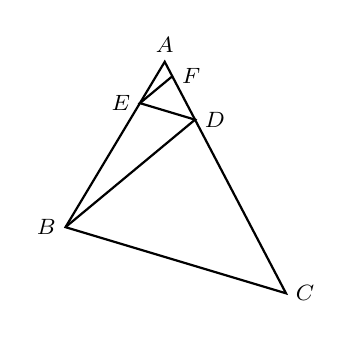
\begin{tikzpicture}[scale=0.7, font=\footnotesize]
	\coordinate (A) at (1,4.2);
	\coordinate (B) at (-0.8,1.2);
	\coordinate (C) at (3.2,0);
	\coordinate (D) at ($(A)!0.25!(C)$);
	\coordinate (E) at ($(A)!0.25!(B)$);
	\coordinate (F) at ($(A)!0.25!(D)$);
	\draw[thick] (A)--(B)--(C)--cycle;
	\draw[thick] (B)--(D)--(E)--(F);
	\node[above] at (A) {$A$};
	\node[left] at (B) {$B$};
	\node[right] at (C) {$C$};
	\node[right] at (D) {$D$};
	\node[left] at (E) {$E$};
	\node[right] at (F) {$F$};
\end{tikzpicture}
\end{document}
